\scanpage{492}
% 492-01: continuation at the upper edge.
and likewise \deleted{$\unsure{\Psi_{-\mathrm j}^{\pi}}$}
\margin{$\left\{
\begin{gathered}
\Psi_{\unsure{-\overline{\mathrm j}|-\mathrm j}}^{\unsure{\pi}}:
\unsure{\widetilde{\Gamma}'_{\mathbb Q}}\simeq
\unsure{\widetilde{\mathcal T}'_{0,3}}
\longrightarrow T_{\rho}(\widehat{\mathbb Z})/\pm1\\
\unsure{\widetilde{\Gamma}'_{\mathbb Q}}
=\{\gamma\in\widetilde{\Gamma}_{\mathbb Q}\mid
\varepsilon_3(\mu)=1,\ \text{where }\mu=\chi(\gamma)\}
\end{gathered}\right.$}
\margin{\unsure{(50}}

% 492-02: upper paragraph and its left margin.
We thus see that the indeterminacies of the \uline{signs} for
$\Theta_{\rho}^{\unsure{\pi}},\Theta_{\sigma}^{\unsure{\pi}}$
correspond precisely to the indeterminacies for $\Theta_G$
itself --- everything hangs together! The latter is removed
\deleted{\unsure{by} \illegible{2}} tautologically when we replace
$\widetilde M_{0,3}$ by the \deleted{\unsure{covering|profinite} \unsure{with|of} $\unsure{2}$ \unsure{sheets}}
\inserted{ad-hoc extension} $\unsure{\widetilde{\mathcal T}_{1,1}}$ by $\pm1$,
so that we find
\margin{We will \unsure{note} \unsure{however} that $\Theta_{\rho}^{\unsure{\pi}}$,
unlike the splitting $\Psi_{\rho}^{\unsure{\pi}}
=\Psi_{1/2}^{\unsure{\pi}}$, is defined on
$\unsure{\widetilde{\mathcal T}_{0,3}}$ in its entirety.
\figure{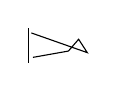
\begin{tikzpicture}
\draw (0,-.22)--(0,.22);
\draw (.04,.16)--(.75,-.09)--(.64,.08)--(.51,-.07)--(.06,-.15);
\end{tikzpicture}}}

% 492-03: display (50).
\[
(50)\qquad \unsure{\widetilde{\mathcal T}_{1,1}}
\longrightarrow \mathrm{GL}(2,\widehat{\mathbb Z})
\]

% 492-04: middle and lower paragraph.
and one should \deleted{\unsure{be able to}} interpret this homomorphism
as the fundamental ``modular'' homomorphism of the theory of elliptic
curves (that the inverse image of \deleted{$\unsure{\Gamma}$}
$\Gamma_{\mathbb Q}\subset\widetilde\Gamma_{\mathbb Q}$ in
$\unsure{\widetilde{\mathcal T}_{1,1}}$ \unsure{can} be interpreted as
$\unsure{\mathcal T_{1,1}}\simeq\pi_1(M_{1,1\,\mathbb Q})$
must be more or less tautological, by construction.)

% 492-05: final paragraph, interlinear addition, and display (51).
It is clear in any case that the two coincide
\inserted{for every $\gamma\in\widetilde M_{0,3}$}
\unsure{viewed} \unsure{as|when} elements of
\[
(51)\qquad \mu_2(\widehat{\mathbb Z})=\{\pm1\}^{\mathbb P}
\qquad (\mathbb P=\text{set of prime numbers})
\]
\mspage{491}

\scanpage{493}
\mspage{549}
% 493-01: continuation, with an overwritten source in the first display.
i.e. they coincide modulo a homomorphism
\[
\deleted{\unsure{M_{0,3}}}\inserted{\unsure{\widetilde\Gamma_{\mathbb Q}}}
\longrightarrow\mu_2(\widehat{\mathbb Z})\simeq\{\pm1\}^{\mathbb P}
\]
i.e. a homomorphism
\[
\begin{aligned}
G_{\mathrm m}(\widehat{\mathbb Z})_2
&=(\widehat{\mathbb Z}^{*})_2\simeq\{\pm1\}^{\mathbb P}
\longrightarrow\deleted{\unsure{\mu}}\unsure{{}_2G_{\mathrm m}}(\widehat{\mathbb Z})
=\mu_2(\widehat{\mathbb Z})\\
&\hspace{24em}\simeq\{\pm1\}^{\mathbb P}
\end{aligned}
\]

% 493-02: middle prose.
--- so it is not a \unsure{certain} indeterminacy that is at issue!
It is morally certain that the two coincide --- I have not tried to
prove it.

% 493-03: lower prose and its interlinear insertion.
As for (35) (36), they must surely correspond to the action of
$\Gamma_{\mathbb Q}$ on the Tate modules of elliptic curves with
exceptional isomorphisms, corresponding precisely to the points
$(1/2,2,-1)$ and $(-\overline{\mathrm j},-\mathrm j)$ of
$M_{0,3\,\mathbb Q}=M_{1,1}[2]'_{\mathbb Q}$.
The indeterminacy of sign \inserted{\unsure{must|of which}} \unsure{correspond|corresponds} to the indeterminacy
in lifting a point of $M_{1,1}[2]'_{\mathbb Q}$ to a point of
$M_{1,1}[2]_{\mathbb Q}$, i.e. in choosing an elliptic curve
(with ``\uline{rigidification}'' of level 2) corresponding to the
\uline{Legendre} data $(0,1,\infty,\unsure{q|\rho})$ with
$\unsure{\rho|q}=1/2$ or $\unsure{\rho|q}=-\overline{\mathrm j}$.
\mspage{492}

\scanpage{494}
% 494-01: upper paragraph.
Even once the \unsure{ambiguity} of sign for
$\Theta_{\unsure{G}}^{\unsure{\pi}}$ is removed by passing to the two-sheeted extension
$\unsure{\widetilde{\mathcal T}_{1,1}}$ of
$\widetilde M_{0,3}$, the indeterminacy of the signs for
$\Theta_{\rho}^{\unsure{\pi}},\Theta_{\sigma}^{\unsure{\pi}}$
is not \unsure{removed} for all that, for the splittings
\deleted{$\unsure{\Psi_{\rho}^{\pi},\Psi_{\sigma}^{\pi}}$}
$\Psi_{1/2}^{\unsure{\pi}},\Psi_{-\overline{\mathrm j}}^{\unsure{\pi}}$)
are not for all that splittings (even partial!)
of \deleted{\unsure{this}} \unsure{the extension}
$\unsure{\widetilde{\mathcal T}_{1,1}}$, but only of
$\widetilde M_{0,3}$ --- and lifting them to splittings of
$\unsure{\widetilde{\mathcal T}_{1,1}}$
\inserted{over $\unsure{\mathcal T_{1,1}}$,}
amounts, very precisely, to choosing precisely elliptic curves with
Legendre rigidification over the points $1/2,-\overline{\mathrm j}$.
Thus, calculations made in terms of automorphisms of the loop groups
$\widehat\Pi_{0,3}$ \unsure{or} \inserted{of}
$\unsure{\mathcal{C}}_{0,3}^{+\wedge}$,
\unsure{give back} \inserted{(without having \unsure{looked for} them!)}
results that fit very closely with particularly crucial
arithmetico-geometric truths.
\mspage{493}

\scanpage{495}
\mspage{550}
% 495-01: heading.
49.\quad \uline{Homomorphisms of} $M_{0,3}$, the general groups
$M_{\rho,\sigma}$.

% 495-02: left-margin notes.
\margin{\unsure{Where we get our feet wet}\ldots}
\margin{\unsure{All of} this section \inserted{I} \unsure{seems}
entirely useless for what follows, it is a preliminary \unsure{groping}
to lead into section \uline{II} page 553.}

% 495-03: first paragraph.
I) Consider a \inserted{closed} subgroup $G$ of $M_{0,3}$,
containing $\unsure{\mathcal C}_{0,3}^{+\wedge}$, hence the inverse image of a
closed subgroup of $\widetilde\Gamma_{0,3}$.
We assume that the latter is ``big enough'' --- say that it contains
a subgroup of finite index in
$\Gamma_{\mathbb Q}\subset\widetilde\Gamma_{0,3}$.
For the moment, we assume for simplicity that $G\subset\operatorname{Ker}\varepsilon_3$.
In summary
\[
(1)\qquad
\unsure{\mathcal C}_{0,3}^{+\wedge}\subset G\subset\widetilde M_{0,3},
\qquad u\in G\Longrightarrow\mu(u)\equiv1\ (3).
\]

% 495-04: interlinear correction and parallel maps.
This last hypothesis thus \deleted{implies}\inserted{means} that
for every $u\in G$, we have $\alpha_0(u)\in\unsure{\mathcal C}_{0,3}^{\wedge+}$,
so we have
\[
(\unsure{2})\qquad
\diagram{\begin{tikzcd}[column sep=large]
G \arrow[r,shift left=.7ex,"\underline{\alpha}_0"]
  \arrow[r,shift right=.7ex,"\underline{\beta}_0"']
& \unsure{\mathcal C}_{0,3}^{+}
\end{tikzcd}},
\]
characterized by
\[
(2')\qquad
\left\{\begin{aligned}
u(\rho)&=\operatorname{int}(\alpha_0)\rho\\
u(\sigma)&=\operatorname{int}(\beta_0)\sigma
\end{aligned}\right.
\qquad
\begin{aligned}
\alpha_0&=\underline{\alpha}_0(u)\\
\beta_0&=\underline{\beta}_0(u).
\end{aligned}
\]

% 495-05: the vertically arranged subgroups, including the intervening sign.
We consider
\[
(3)\qquad
\begin{array}{l}
G(0)=G\cap\widetilde M_{0,3}(0)\\[-.4em]
\quad\cap\\[-.4em]
G[0]=G\cap\widetilde M_{0,3}[0]=\operatorname{Norm}_{G}(L_0^{\unsure{\mathcal C}})
\end{array}
\]
so that
\[
\begin{aligned}
(4)\qquad&G=G(0).\unsure{\mathcal C}_{0,3}^{+\wedge}
&&\text{(semidirect product)}\\
(5)\qquad&G[0]=G(0).L_0^{\unsure{\mathcal C}}
&&\text{id}\\
(6)\qquad&G[0]\cap\unsure{\mathcal C}_{0,3}^{+\wedge}
=L_0^{\unsure{\mathcal C}}.
\end{aligned}
\]

% 495-06: definition (7) and last line.
We have set
\[
(7)\qquad
\begin{gathered}
L_0^{\unsure{\mathcal C}}=\text{closed subgroup of }
\unsure{\mathcal C}_{0,3}^{+\wedge}\text{ generated}\\
\text{by }\varepsilon_0
\end{gathered}
\]
and we define likewise $L_1^{\unsure{\mathcal C}},L_{\infty}^{\unsure{\mathcal C}}$.
\mspage{494}

\scanpage{496}
% 496-01: paragraph and first map, with changes of target notation.
Consider a \inserted{profinite} group
$\deleted{\unsure{A}}\inserted{M}$, and a \inserted{(continuous)}
\uline{surjective} homomorphism
\[
(8)\qquad \varphi:G\longrightarrow\deleted{\unsure{A}}M.
\]
We set
\[
(9)\quad
\left\{\begin{aligned}
\varphi(\unsure{\mathcal C}_{0,3}^{+\wedge})
 &=\unsure{\mathcal C}\qquad\text{normal subgroup of }M\\
\varphi(G(0))&=\deleted{\unsure{A}}\inserted{M}(0)\\
\varphi(G[0])&=\deleted{\unsure{A}}\inserted{M}[0].\\
\varphi(L_0^{\unsure{\mathcal C}})&=L_0^{\deleted{\unsure{\mathcal C}}}
\end{aligned}\right.
\]

% 496-02: subgroup relations.
\deleted{\unsure{Thus}}

Thus these are closed subgroups of $M$, satisfying
\[
\begin{aligned}
(10)\qquad&M(0)\subset M[0]\subset\operatorname{Norm}_{M}(L_0)\\
(11)\qquad&L_0^{\deleted{\unsure{\mathcal C}}}
\subset\unsure{\mathcal C}\cap M[0].
\end{aligned}
\]

% 496-03: the surviving generator relations.
By abuse of language, we still denote by $\rho,\sigma,\varepsilon_0,\varepsilon_1$
\ldots\ the images of these elements in $\unsure{\mathcal C}$, which
therefore satisfy there the relations known in $\unsure{\mathcal C}_{0,3}^{+\wedge}$,
in particular
\[
(12)\qquad
\sigma^2=\rho^3=1,\qquad
\sigma\rho=\varepsilon_0,\quad \rho\sigma=\varepsilon_1,\qquad
\varepsilon_1=\sigma(\varepsilon_0)=\rho(\varepsilon_0).
\]

% 496-04: paragraph and revised definition (13).
The restrictions of the maps $\alpha_0,\beta_0$ of (2,2') to
$M_{\rho,\sigma}[0]$ will rather be denoted $\alpha,\beta$, where $\alpha,\beta$
are in fact maps
\[
(13)\quad
\diagram{\begin{tikzcd}[column sep=large]
{\begin{gathered}
SG\overset{\mathrm{dfn}}=\deleted{\text{extension of}}\ G\\
\text{by }L_0^{\unsure{\mathcal C}},\ \text{inverse}\\
\text{image of }\unsure{G}\\
\text{in }S\widetilde M_{0,3}\\
=\{(u,f)\in G\times\unsure{\mathcal C}_{0,3}^{+\wedge}\mid fu\in G[0]
\end{gathered}}
\arrow[r,shift left=.7ex,"\alpha"]
\arrow[r,shift right=.7ex,"\beta"']
&\unsure{\mathcal C}_{0,3}^{+\wedge}
\end{tikzcd}}
\]
of which we look at the restrictions to the \uline{subgroup}
($\simeq M_{\rho,\sigma}[0]$) of $SG$ defined by the relation $f=1$.

% 496-05: composition of the two functions, and (14).
Composing $\underline\alpha,\underline\beta:$
\diagram{\begin{tikzcd}[column sep=small]
\deleted{\unsure{M[0]}}\inserted{G[0]}
\arrow[r,shift left=.5ex]\arrow[r,shift right=.5ex]
&\unsure{\mathcal C}_{0,3}^{+\wedge}
\end{tikzcd}}
with $\varphi\mid\unsure{\mathcal C}_{0,3}^{+\wedge}$, we find
maps, again denoted $\underline\alpha,\underline\beta$
(where $\underline\alpha^M,\underline\beta^M$ in case of possible confusion)
\[
(14)\qquad
\diagram{\begin{tikzcd}[column sep=large]
G[0]\arrow[r,shift left=.7ex,"\underline\alpha"]
\arrow[r,shift right=.7ex,"\underline\beta"']
&\unsure{\mathcal C}
\end{tikzcd}}
\]
thus satisfying
\[
(15)\qquad
\left\{\begin{aligned}
\unsure{u}(\rho)&=\operatorname{int}(\alpha)\rho\\
\unsure{u}(\sigma)&=\operatorname{int}(\beta)\sigma
\end{aligned}\right.
\qquad
\begin{gathered}
\text{for }u\in M[0]\ \inserted{\text{\unsure{of}}}\text{ the form }\varphi(u_0),\\
\text{and }\alpha=\underline\alpha(u_0),\ \beta=\underline\beta(u_0).
\end{gathered}
\]
\mspage{495}